\begin{figure}[h!]
    \centering
    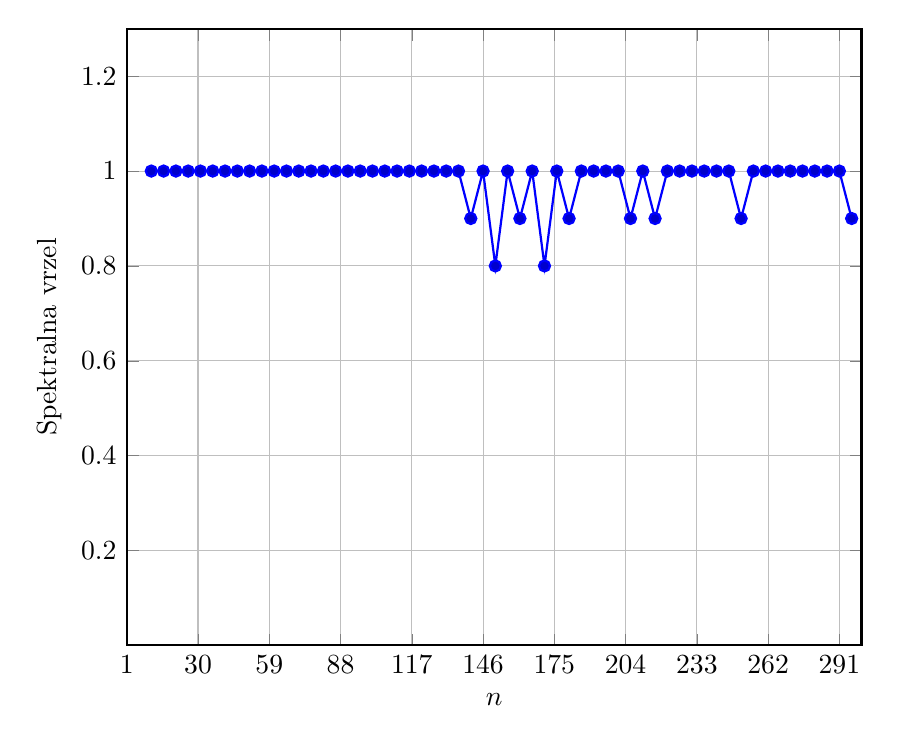
\begin{tikzpicture}
        \begin{axis}[
                xlabel={$n$},
                width=0.9\textwidth,
                ylabel={Spektralna vrzel},
                grid=major,
                ymin=0, ymax=1.3,
                xmin=1, xmax=300,
                xtick={1,30,...,300},
                ytick={0.2,0.4,0.6,0.8,1,1.2},
                thick
            ]
            \addplot coordinates {
                (11, 1)
                (16, 1)
                (21, 1)
                (26, 1)
                (31, 1)
                (36, 1)
                (41, 1)
                (46, 1)
                (51, 1)
                (56, 1)
                (61, 1)
                (66, 1)
                (71, 1)
                (76, 1)
                (81, 1)
                (86, 1)
                (91, 1)
                (96, 1)
                (101, 1)
                (106, 1)
                (111, 1)
                (116, 1)
                (121, 1)
                (126, 1)
                (131, 1)
                (136, 1)
                (141, 0.9)
                (146, 1)
                (151, 0.8)
                (156, 1)
                (161, 0.9)
                (166, 1)
                (171, 0.8)
                (176, 1)
                (181, 0.9)
                (186, 1)
                (191, 1)
                (196, 1)
                (201, 1)
                (206, 0.9)
                (211, 1)
                (216, 0.9)
                (221, 1)
                (226, 1)
                (231, 1)
                (236, 1)
                (241, 1)
                (246, 1)
                (251, 0.9)
                (256, 1)
                (261, 1)
                (266, 1)
                (271, 1)
                (276, 1)
                (281, 1)
                (286, 1)
                (291, 1)
                (296, 0.9)
                };
        \end{axis}
    \end{tikzpicture}
    \caption{Graf proporcije Ramanujanovih grafov od 1 do 300}
\end{figure}

\begin{figure}[h!]
    \centering
    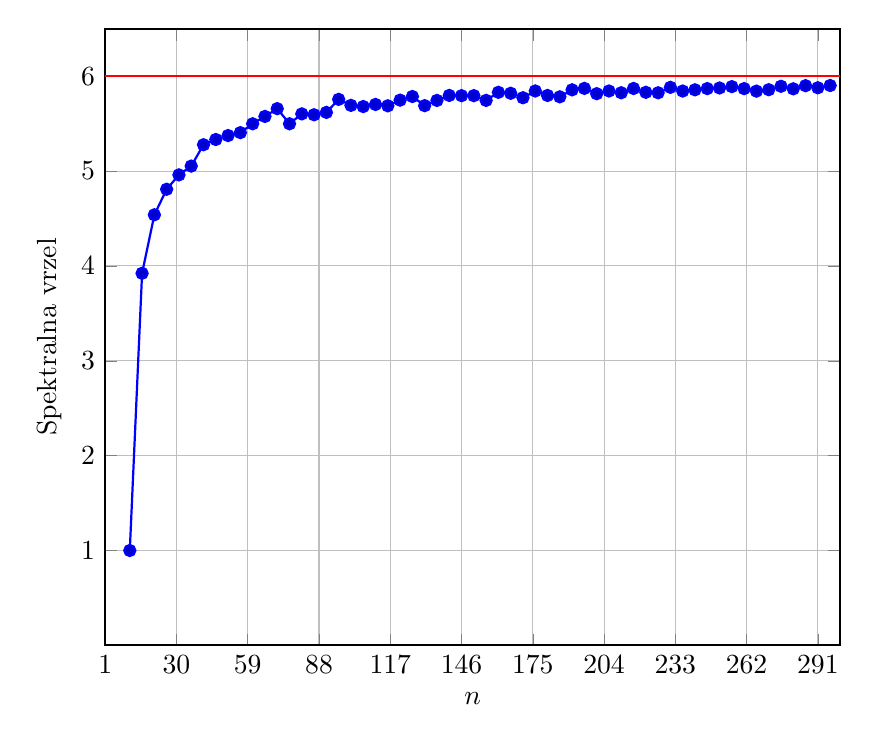
\begin{tikzpicture}
        \begin{axis}[
                xlabel={$n$},
                width=0.9\textwidth,
                ylabel={Spektralna vrzel},
                grid=major,
                ymin=0, ymax=6.5,
                xmin=1, xmax=300,
                xtick={1,30,...,300},
                ytick={1,2,3,4,5,6},
                thick
            ]
            \addplot coordinates {
                (11, 1.000000000000002)
                (16, 3.9222400439343685)
                (21, 4.538860013159836)
                (26, 4.808216830193524)
                (31, 4.959790573039687)
                (36, 5.052688498284467)
                (41, 5.277523254626809)
                (46, 5.332807138620655)
                (51, 5.37442486437986)
                (56, 5.405097185918946)
                (61, 5.498571934186495)
                (66, 5.575938409277276)
                (71, 5.657944175537072)
                (76, 5.498418778423789)
                (81, 5.602860389811621)
                (86, 5.593469989602875)
                (91, 5.6184462225220955)
                (96, 5.755892359656839)
                (101, 5.692360968966922)
                (106, 5.680076900644869)
                (111, 5.702246521366402)
                (116, 5.687849569151763)
                (121, 5.7477099188934355)
                (126, 5.786041727310356)
                (131, 5.689452187703263)
                (136, 5.744546954992545)
                (141, 5.797192510119292)
                (146, 5.794721314474317)
                (151, 5.794856354446884)
                (156, 5.7450428693297475)
                (161, 5.830087183980121)
                (166, 5.819987775195498)
                (171, 5.773037906395612)
                (176, 5.8442881137227465)
                (181, 5.796921259614794)
                (186, 5.7826092969682374)
                (191, 5.856437633170694)
                (196, 5.871746814293452)
                (201, 5.815647264915688)
                (206, 5.844111155403364)
                (211, 5.82553111614388)
                (216, 5.870565933769311)
                (221, 5.830291882849532)
                (226, 5.825318465358029)
                (231, 5.8827281797714175)
                (236, 5.84361148217756)
                (241, 5.856540765886825)
                (246, 5.869304300978469)
                (251, 5.8758368544626185)
                (256, 5.890130266065601)
                (261, 5.8691466815061935)
                (266, 5.842566144716664)
                (271, 5.857769806232399)
                (276, 5.893678696498535)
                (281, 5.866955967785748)
                (286, 5.89999683489138)
                (291, 5.878019228343736)
                (296, 5.901828771475102)
                };
                \addplot[red, thick] coordinates {(0, 6) (300, 6)};
        \end{axis}
    \end{tikzpicture}
    \caption{Graf spektralnih vrzeli za \(n\) od 1 do 300}
\end{figure}

